\documentclass[12pt]{decar-wsd}    % Document style

\usepackage{lastpage}
\usepackage{decar-common}    % Commonly used commands and packages
\usepackage{decar-dynamics}  % Dynamics commands (load only if needed)
\usepackage{decar-lie}       % Lie group commands (load only if needed)
\usepackage{todonotes}        % Load whatever other packages you want here
\usepackage{decar-post}      % Packages that must be loaded last
\usepackage{amsmath}
\usepackage{amssymb}
% Reset equation numbers at each section
\usepackage{chngcntr}
% \usepackage{lastpage}

\newcommand{\minus}{\ominus}
\newcommand{\plus}{\oplus}
\newcommand{\del}{\partial}
\newcommand{\dxi}{\delta \mbs{\xi}}
\newcommand{\nav}{\mathrm{nav}}
\newcommand{\Hessdx}[1]{\frac{\del^2 #1}{\del \mbf{x} \del \mbf{x}^\trans}}
\newcommand{\Jacdx}[1]{\frac{\del #1}{\del \mbf{x}}}
\newcommand{\JacdxT}[1]{\frac{\del #1}{\del \mbf{x}^\trans}}
\newcommand{\kmax}{{k^*}}
\newcommand{\ErrDim}{{n_\textrm{e}}}
\newcommand{\Dee}{D}
\newcommand{\StateDim}{{n_\textrm{x}}}
\newcommand{\LogSumExp}{{\textrm{LogSumExp}}}
\newcommand{\Gaussian}[1]{\mc{N}\left(#1\right)}
\newcommand{\HessianGen}{\mc{H}}

\newcommand{\LiwLandmark}{{l_\LiwLandmarkIdx}}
\newcommand{\LiwTimeIdx}{i}
\newcommand{\ErrJacSolver}{\mbf{J}}
\newcommand{\GmmNormConst}[1]{{\gamma_{\text{#1}}}}
\newcommand{\NumComp}{{n_k}}
\newcommand{\MonomialsToDegree}[2]{[#1]_{#2}}
\newcommand{\SparseMonomialsToDegree}[2]{[#1]_{#2, s}}
\newcommand{\mbsxi}{{\mbs{\xi}}}
\newcommand{\lndmrk}{{\mbs{\ell}}}
\newcommand{\mbsXi}{{\mbs{\Xi}}}
\newcommand{\mbstheta}{{\mbs{\theta}}}
\newcommand{\mbsTheta}{{\mbs{\Theta}}}
\newcommand{\mbslambda}{{\mbs{\lambda}}}
\newcommand{\MomentMatrix}{{\mbf{M}}}
\newcommand{\slice}[1]{{\textrm{slice}(#1)}}
\newcommand{\Symmetrize}[1]{{\textrm{Symm}\left(#1\right)}}
\newcommand{\InnerProduct}[2]{{\left \langle #1, #2\right \rangle}}
\newcommand{\SetSymbol}{{\mc{S}}}
\newcommand{\SuchThat}{{\text{s.t.}}}
\newcommand{\Value}{{\text{val}}}
\newcommand{\PositiveSemidefiniteGeq}{{\ \succcurlyeq \ }}
\newcommand{\OneVariable}{{1}}
\newcommand{\Certificate}[1]{\mc{C}\left(#1\right)}
\newcommand{\NumConstraints}{{n_{\text{constr.}}}}
\newcommand{\ConstraintSet}{{\mc{A}}}
\newcommand{\matvec}[1]{\text{vec}\left(#1\right)}
\newcommand{\PsdMatrixSet}[1]{{\mathbb{S}_{+}^{#1}}}
\newcommand{\PdMatrixSet}[1]{{\mathbb{S}_{++}^{#1}}}
\newcommand{\spacespan}{{\text{span}}}
\newcommand{\kron}{{\ \otimes \ }}
\newcommand{\vech}[1]{{\text{vech}\left(#1\right)}}
\newcommand{\vecmat}[1]{{\text{vec}\left(#1\right)}}
\renewcommand{\vec}[1]{{\text{vec}\left(#1\right)}}
\newcommand{\parenth}[1]{{\left(#1\right)}}
\usepackage[nocomma]{optidef}
\DeclareMathOperator{\Exp}{Exp}
\DeclareMathOperator{\Log}{Log}

\renewcommand{\theequation}{\arabic{equation}}

\hypersetup{
    colorlinks=true,   
    urlcolor=cyan,
    }

\addbibresource{library.bib} % Bibtex file containing the references

\title{Kalman Filter Exercise}
\author{Irene Simier}

\begin{document}

\maketitle
\section{Mass-spring-damper System}

\begin{figure}[h]
    \centering
    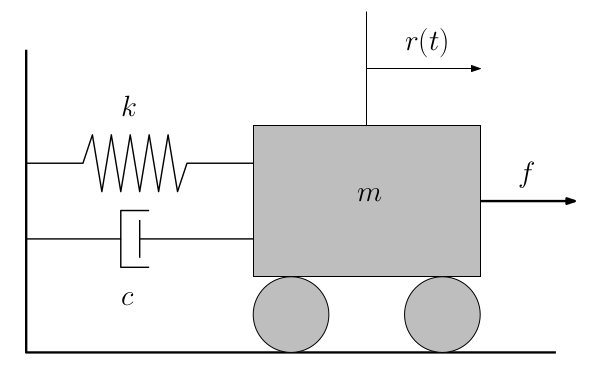
\includegraphics[width=0.6\textwidth]{figures/mass_spring_damper.png}
    \caption{Mass-spring-damper system.}
    \label{fig:mass_spring_damper}
\end{figure}

Figure~\ref{fig:mass_spring_damper} shows a mass-spring-damper system, 
consisting of a mass \( m \) attached to a spring with spring constant \( k \), 
a dashpot with damping constant \( c \), and also subject to an external force \( f(t) \). 
The position of the cart from its equilibrium position is denoted as \( r(t) \), 
which is a function of time \( t \).

The equation of motion of the cart is given by

\begin{align}
    \ddot{r}(t) + c\dot{r}(t) + kr(t) = f(t)
\end{align}
\clearpage

\subsection{No external Force}

With no external force, the equation of motion becomes

\begin{align}
    \ddot{r}(t) + c\dot{r}(t) + kr(t) = 0 \\
    \ddot{r}(t) = \frac{1}{m}(-k r(t) - c \dot{r}(t))
\end{align}

The state-space form is given by
 
\begin{equation}
    \begin{aligned}
        \dot{\mathbf{x}}(t) &= 
        \begin{bmatrix}
            0 & 1 \\
            -\dfrac{k}{m} & -\dfrac{c}{m}
        \end{bmatrix}
        \mathbf{x}(t), \quad\quad
        \mathbf{x}(t) = 
        \begin{bmatrix}
            r(t) \\
            \dot{r}(t)
        \end{bmatrix}
    \end{aligned}
    \end{equation}

\subsection{Non-zero external Force}

Let \( f(t) = A \sin(\omega t) \), the equation of motion becomes:

\begin{align}
    \ddot{r}(t) + c\dot{r}(t) + k r(t) = A \sin(\omega t)
\end{align}

The state-space form is given by
    
\begin{equation}
    \begin{aligned}
        \dot{\mathbf{x}}(t) &= 
        \begin{bmatrix}
            0 & 1 \\
            -\dfrac{k}{m} & -\dfrac{c}{m}
        \end{bmatrix}
        \mathbf{x}(t) + 
        \begin{bmatrix}
            0 \\
            -\dfrac{1}{m}
        \end{bmatrix}
        \mathbf{u}(t), \quad\quad
        \mathbf{x}(t) = 
        \begin{bmatrix}
            r(t) \\
            \dot{r}(t)
        \end{bmatrix}, \;
        \mathbf{u}(t) = A sin(wt)
    \end{aligned}
    \end{equation}
    
\section{Sensor Measurements}

In this system, we use two sensors to measure the position 
and acceleration of the mass.

The acceleration measurement, denoted \( u_{\text{acc}}(t) \), 
is given by

\begin{equation}
    \begin{aligned}
        u_{\text{acc}}(t) &= \ddot{r}(t) + w(t), 
        \quad\quad w(t) \sim \mathcal{N}(0, Q(t)) \\
        u_{\text{acc}}(t) &= \frac{1}{m} \left( f(t) - k r(t) - c \dot{r}(t) \right) + w(t), 
    \end{aligned}
    \label{eq:acc_measurement}
\end{equation}


where \( w(t) \) is zero-mean Gaussian noise with time-varying 
covariance \( Q(t) \).
\clearpage

The position sensor provides a noisy measurement of the true position:

\begin{equation}
    y(t) = r(t) + v(t),
    \quad\quad v(t) \sim \mathcal{N}(0, R(t))
    \label{eq:pos_measurement}
\end{equation}

where \( v(t) \) is zero-mean Gaussian noise with covariance \( R(t) \).

Together, these measurements are used for state estimation in 
filtering and control algorithms.
\section{Continuous Time System}

Since acceleration is measured directly, we can simplify the model 
to a kinematic relation:

\begin{equation}
\ddot{r}(t) = u_{\text{acc}}(t)
\label{eq:kinematics}
\end{equation}

This allows us to avoid modeling the full mass-spring-damper dynamics 
involving forces and mass.

The state-space form is now given by
    
\begin{equation}
    \dot{\mathbf{x}}(t) = 
    \begin{bmatrix}
    0 & 1 \\
    0 & 0
    \end{bmatrix}
    \mathbf{x}(t) +
    \begin{bmatrix}
    0 \\
    1
    \end{bmatrix}
    u_{\text{acc}}(t)
    \label{eq:continuous_system}
\end{equation}

\begin{equation}
    \begin{aligned}
        y(t) &= 
        \begin{bmatrix}
            1 & 0
        \end{bmatrix}
        \mathbf{x}(t) + v(t)
    \end{aligned}
\end{equation}
    
\section{Discretization}

Using a Zero-Order-Hold (ZOH) discretization, the continuous-time system is converted into 
the following discrete-time state-space form:

\begin{align}
    \mathbf{x}_k &= A_{k-1} \, \mathbf{x}_{k-1} + B_{k-1} \, a_{k-1} + \mathbf{w}_{k-1}, \quad \mathbf{w}_{k-1} \sim \mathcal{N}(0, Q_{k-1}) \\
    y_k &= r_k + v_k, \quad\quad\quad\quad\quad\quad\quad\quad\quad\quad\quad v_k \sim \mathcal{N}(0, R_k)
\end{align}

Here, \( \mathbf{x}_k \in \mathbb{R}^2 \) is the discrete-time state vector representing position and velocity,  
\( a_{k-1} \) is the sampled acceleration input, and  \( y_k \) is the noisy position measurement.
\( R_k \) is defined by the position sensor noise model.

The matrices \( A_{k-1} \), \( B_{k-1} \) and \( Q_{k-1} \)  are derived by discretizing the continuous-time 
system in equation \(\ref{eq:continuous_system}\). The process is as follows:

\clearpage

\textbf{Step 1: Compute \( A_d \) and \( B_d \) using ZOH}

\begin{align}
    M_{\text{zoh}} &= \begin{bmatrix}
    A & B \\
    0 & 0
    \end{bmatrix} \cdot \Delta t \\
    \begin{bmatrix} A_d & B_d \end{bmatrix} &= \exp(M_{\text{zoh}})
\end{align}

The process noise covariance \( Q_{k-1} \) can be computed using Van Loan’s method.

\textbf{Step 2: Compute \( Q_k \) using Van Loan's method}

\begin{align}
    M_{\text{vl}} &= \begin{bmatrix}
    -A & (L Q_c L^T) \\
    0 & A^T
    \end{bmatrix} \cdot \Delta t \\
    \Phi &= \exp(M_{\text{vl}}) \\
    Q_k &= A_d \cdot \Phi_{12}
\end{align}
\section{Kalman Filter}

The Kalman filter is applied to estimate the state \( \mathbf{x}(t) \) 
of the system by combining the predicted state from the accelerometer data
with the corrected state from the position measurements.

\subsection{Algorithm}

\textbf{Step 1: Initialization}

The initial state estimate \( \hat{\mathbf{x}}_0 \) is typically set to the expected 
initial position and velocity, i.e., \( \hat{\mathbf{x}}_0 = \mathbb{E}[\mathbf{x}_0] \). 
The initial state covariance \( P_0 \) represents the uncertainty in the initial estimate 
and is usually set to a large value to reflect high uncertainty about the initial state.

\begin{align}
    \hat{\mathbf{x}}_0 &= \mathbb{E}[\mathbf{x}_0] \\
    P_0 &= \mathbb{E}[(\mathbf{x}_0 - \hat{\mathbf{x}}_0)(\mathbf{x}_0 - \hat{\mathbf{x}}_0)^T]
\end{align}

\textbf{Step 2: Prediction Step}

In the prediction step, the state is predicted using the previous state 
estimate and the measured acceleration \( a_k \):

\begin{align}
    \mathbf{x}_{k|k-1} &= A \mathbf{x}_{k-1|k-1} + B a_k \\
    P_{k|k-1} &= A P_{k-1|k-1} A^T + Q
\end{align}

\textbf{Step 3: Update Step}

In the update step, the state estimate is corrected using the position measurement \( y_k \):

\begin{align}
    S_k &= C P_{k|k-1} C^T + R \\
    K_k &= P_{k|k-1} C^T S_k^{-1} \\
    \mathbf{x}_{k|k} &= \mathbf{x}_{k|k-1} + K_k (y_k - C \mathbf{x}_{k|k-1}) \\
    P_{k|k} &= (I - K_k C) P_{k|k-1} (I - K_k C)^T + K_k R K_k^T
\end{align}

\subsection{Simulation Results}

The accelerometer data (\( a_k \)) and position measurements (\( y_k \)) 
were obtained at discrete time steps. Both measurements are sampled at the 
same frequency, with the sampling interval \( \Delta t = 0.01 \, \text{s} \) 
(100 Hz sampling rate). The following values were used to generate the figure:

\textbf{Physical Parameters:}
\begin{itemize}
    \item Mass: \( m = 1.0 \, \text{kg} \)
    \item Damping coefficient: \( c = 0.5 \, \text{N·s/m} \)
    \item Spring constant: \( k = 5.0 \, \text{N/m} \)
    \item External force: \( f(t) = A \sin(\omega t) \), where 
    \( A = 5 \, \text{N} \) and \( \omega = 2\pi \, \text{rad/s} \)
\end{itemize}

\textbf{Covariance:}
\begin{itemize}
    \item Process noise covariance: \( Q_k = 0.1 \)
    \item Measurement noise covariance for position: \( R_k = 0.05 \)
    \item Initial state covariance: 
    \[
    P_0 =
    \begin{bmatrix}
    0.1 & 0 \\
    0 & 0.1
    \end{bmatrix}
    \]
\end{itemize}

\textbf{Initial State:}
\begin{itemize}
    \item Initial position and velocity: 
    \[
    \mathbf{x}_0 = \begin{bmatrix} 5 \\ 0 \end{bmatrix} \quad \text{(initial position = 5 m, initial velocity = 0 m/s)}
    \]
\end{itemize}

The Kalman filter was applied to estimate the position and velocity  
of the system using noisy accelerometer and position measurements.  
The result, shown in Figure \ref{fig:kf_same_freq}, combines the  
predicted state from the accelerometer data with the corrected state  
from the position measurements.

\begin{figure}[H]
    \centering
    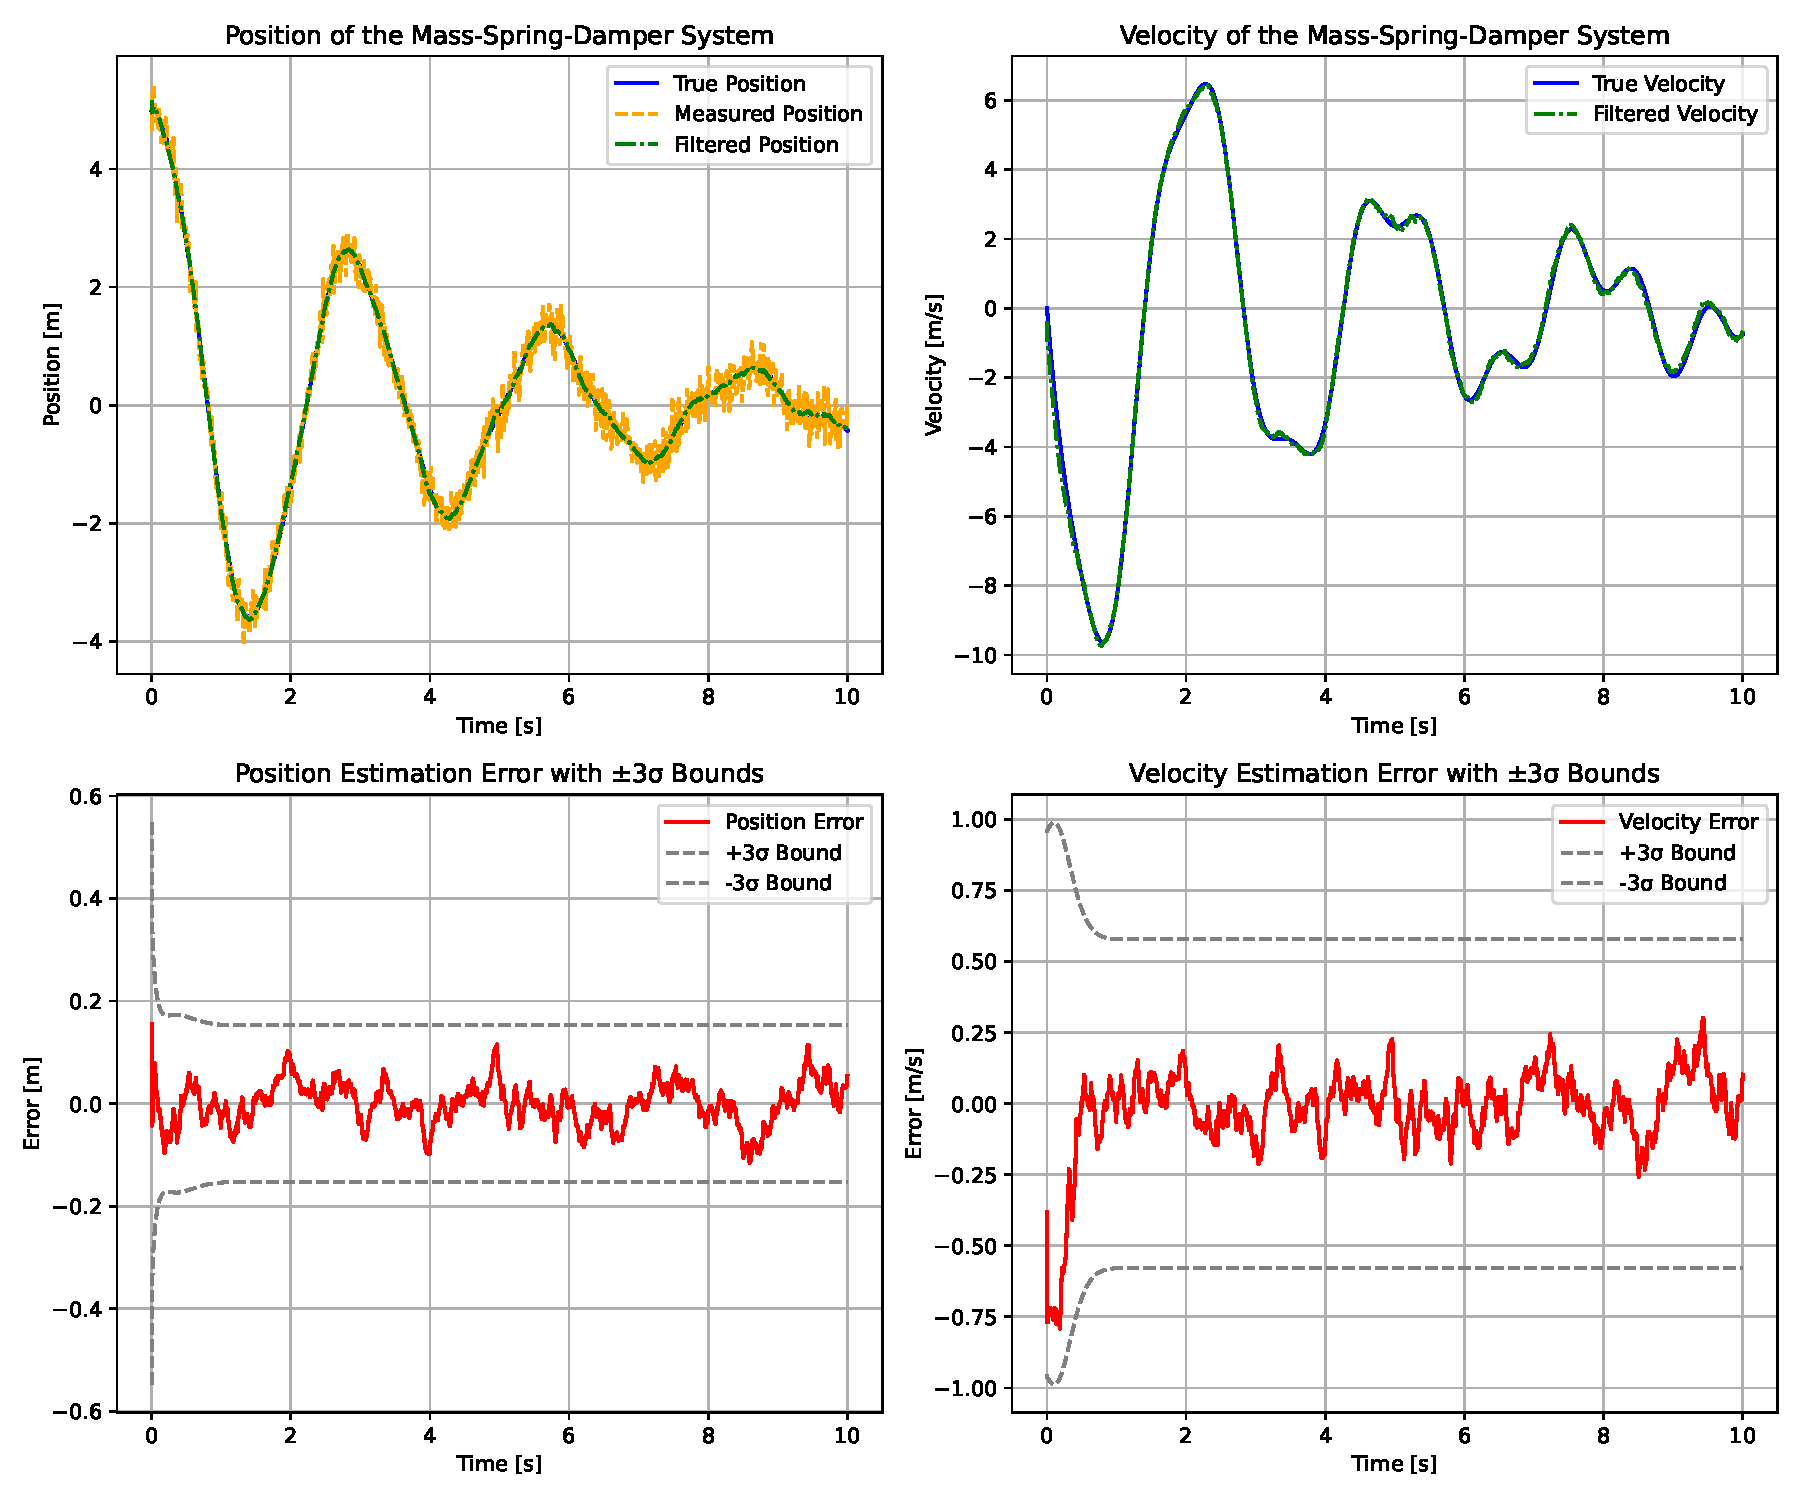
\includegraphics[width=1\textwidth]{figures/kf_same_freq.pdf}
    \caption{Kalman filter estimation with accelerometer and position measurements at the same frequency. The plots show the true, measured, and filtered values for position and velocity, as well as the errors with $\pm 3\sigma$ bounds.}
    \label{fig:kf_same_freq}
\end{figure}

The figure above demonstrates the performance of the Kalman filter when both accelerometer  
and position measurements are sampled at the same frequency. The filter effectively fuses  
the two sources to provide accurate estimates with uncertainty bounds.

In Figure \ref{fig:kf_freq_50}, the accelerometer data is sampled 50 times more frequently  
than the position measurements. Between two position updates, the filter relies solely on  
the accelerometer data to predict the state. This causes the state covariance to increase as  
uncertainty accumulates. When a position measurement becomes available, the update step  
reduces the uncertainty, resulting in a drop in the covariance. This cycle repeats, and the  
error bounds expand and contract periodically, reflecting the alternating prediction-only  
and correction phases.

\begin{figure}[H]
    \centering
    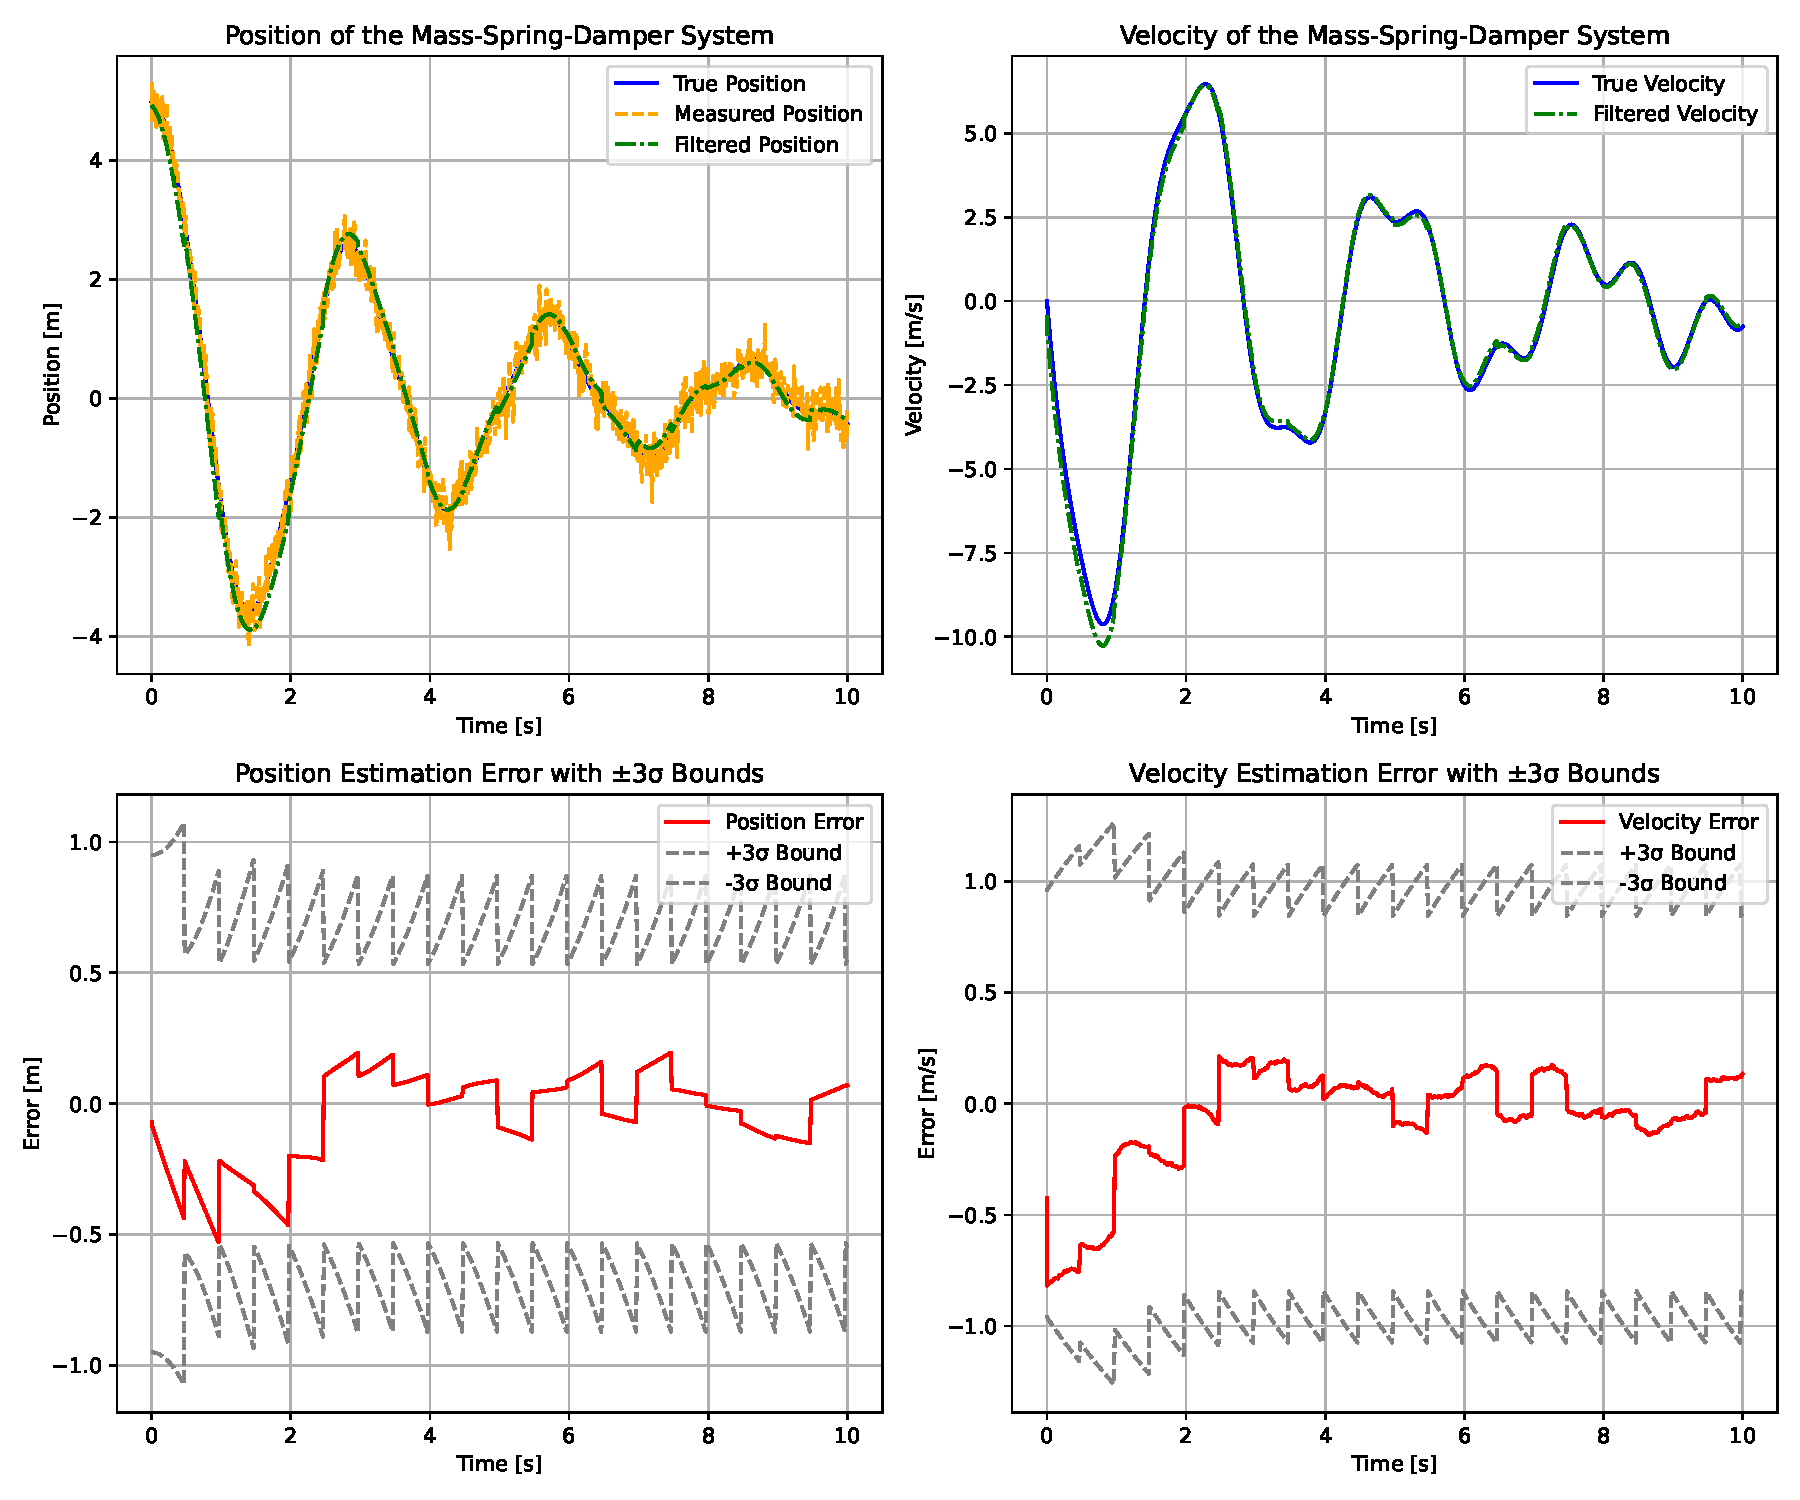
\includegraphics[width=1\textwidth]{figures/kf_freq_50.pdf}
    \caption{Kalman filter estimation where the accelerometer is sampled 50 times more frequently than the position sensor.}
    \label{fig:kf_freq_50}
\end{figure}


\section{Extended Kalman Filter}

We now consider a scenario where the position is not measured directly. Instead, a distance sensor measures the Euclidean distance from the cart to a fixed point on a wall located at a horizontal offset \( d \) and vertical height \( h \) above the cart's equilibrium position. 

\begin{align}
    g(\mathbf{x}_k) = \sqrt{(r_k + d)^2 + h^2}
\end{align}

Since the measurement model is nonlinear, we use an Extended Kalman Filter (EKF) to linearize the measurement model around the predicted state at each time step.

\clearpage

\subsection{System Model and Linearization}

The process model remains unchanged since acceleration is still measured directly:

\begin{align}
    \mathbf{x}_k &= A_{k-1} \, \mathbf{x}_{k-1} + B_{k-1} \, a_{k-1} + \mathbf{w}_{k-1}, \quad \mathbf{w}_{k-1} \sim \mathcal{N}(0, Q_{k-1})
\end{align}

However, the measurement model changes due to the new sensor. 

\begin{align}
    y_k &= g(\mathbf{x}_k) + v_k, \quad\quad
    v_k \sim \mathcal{N}(0, R_k) 
\end{align}

The Jacobian \( C_k \) of the nonlinear measurement model at each time step is:


\begin{align}
    C_k = \frac{\partial g}{\partial \mathbf{x}} |_{\hat{\mathbf{x}}_{k|k-1}} =
    \begin{bmatrix}
        \dfrac{\hat{r}_{k|k-1} + d}{\sqrt{(\hat{r}_{k|k-1} + d)^2 + h^2}} & 0
    \end{bmatrix}
\end{align}

This Jacobian captures the sensitivity of the measurement to the state and is used in the EKF to compute the Kalman gain and update the estimate.

\subsection{Algorithm}

\textbf{Step 1: Initialization}

The initial state estimate \( \hat{\mathbf{x}}_0 \) is typically set to the expected 
initial position and velocity, i.e., \( \hat{\mathbf{x}}_0 = \mathbb{E}[\mathbf{x}_0] \). 
The initial state covariance \( P_0 \) represents the uncertainty in the initial estimate.

\begin{align}
    \hat{\mathbf{x}}_0 &= \mathbb{E}[\mathbf{x}_0] \\
    P_0 &= \mathbb{E}[(\mathbf{x}_0 - \hat{\mathbf{x}}_0)(\mathbf{x}_0 - \hat{\mathbf{x}}_0)^T]
\end{align}

\textbf{Step 2: Prediction Step}

In the prediction step, the state is predicted using the previous state 
estimate and the measured acceleration \( a_k \):

\begin{align}
    \mathbf{x}_{k|k-1} &= A \mathbf{x}_{k-1|k-1} + B a_k \\
    P_{k|k-1} &= A P_{k-1|k-1} A^T + Q
\end{align}

\clearpage

\textbf{Step 3: Update Step}


In the update step, the state estimate is corrected using the nonlinear measurement model. To apply the EKF, we linearize this measurement function. The Jacobian matrix \( C \) is computed as the derivative of \( g(\mathbf{x}) \) with respect to the state vector \( \mathbf{x} \):

\begin{align}
    C &= \frac{\partial g(\mathbf{x})}{\partial \mathbf{x}} \\
    S_k &= C P_{k|k-1} C^T + R \\
    K_k &= P_{k|k-1} C^T S_k^{-1} \\
    \mathbf{x}_{k|k} &= \mathbf{x}_{k|k-1} + K_k \left( y_k - g(\mathbf{x}_{k|k-1}) \right) \\
    P_{k|k} &= (I - K_k C) P_{k|k-1} (I - K_k C)^T + K_k R K_k^T
\end{align}

\subsection{Simulation Results}

The simulation uses the same system parameters as in the standard Kalman filter case. Regarding the distance measurement, the wall is located at a distance \( d = 5 \, \text{m} \) from the equilibrium position of the cart and at a height \( h = 5 \, \text{m} \).

Figure~\ref{fig:ekf} below shows the performance of the Extended Kalman Filter (EKF) when the position of the cart is not directly measured. The EKF is able to estimate both position and velocity accurately despite the nonlinear observation model. As shown in the plots, the filter effectively tracks the true position and velocity of the mass-spring-damper system. The estimation errors remain within the \( \pm 3\sigma \) confidence bounds, indicating that the EKF is well-tuned and the uncertainty estimates are consistent with the actual errors.

\begin{figure}[H]
    \centering
    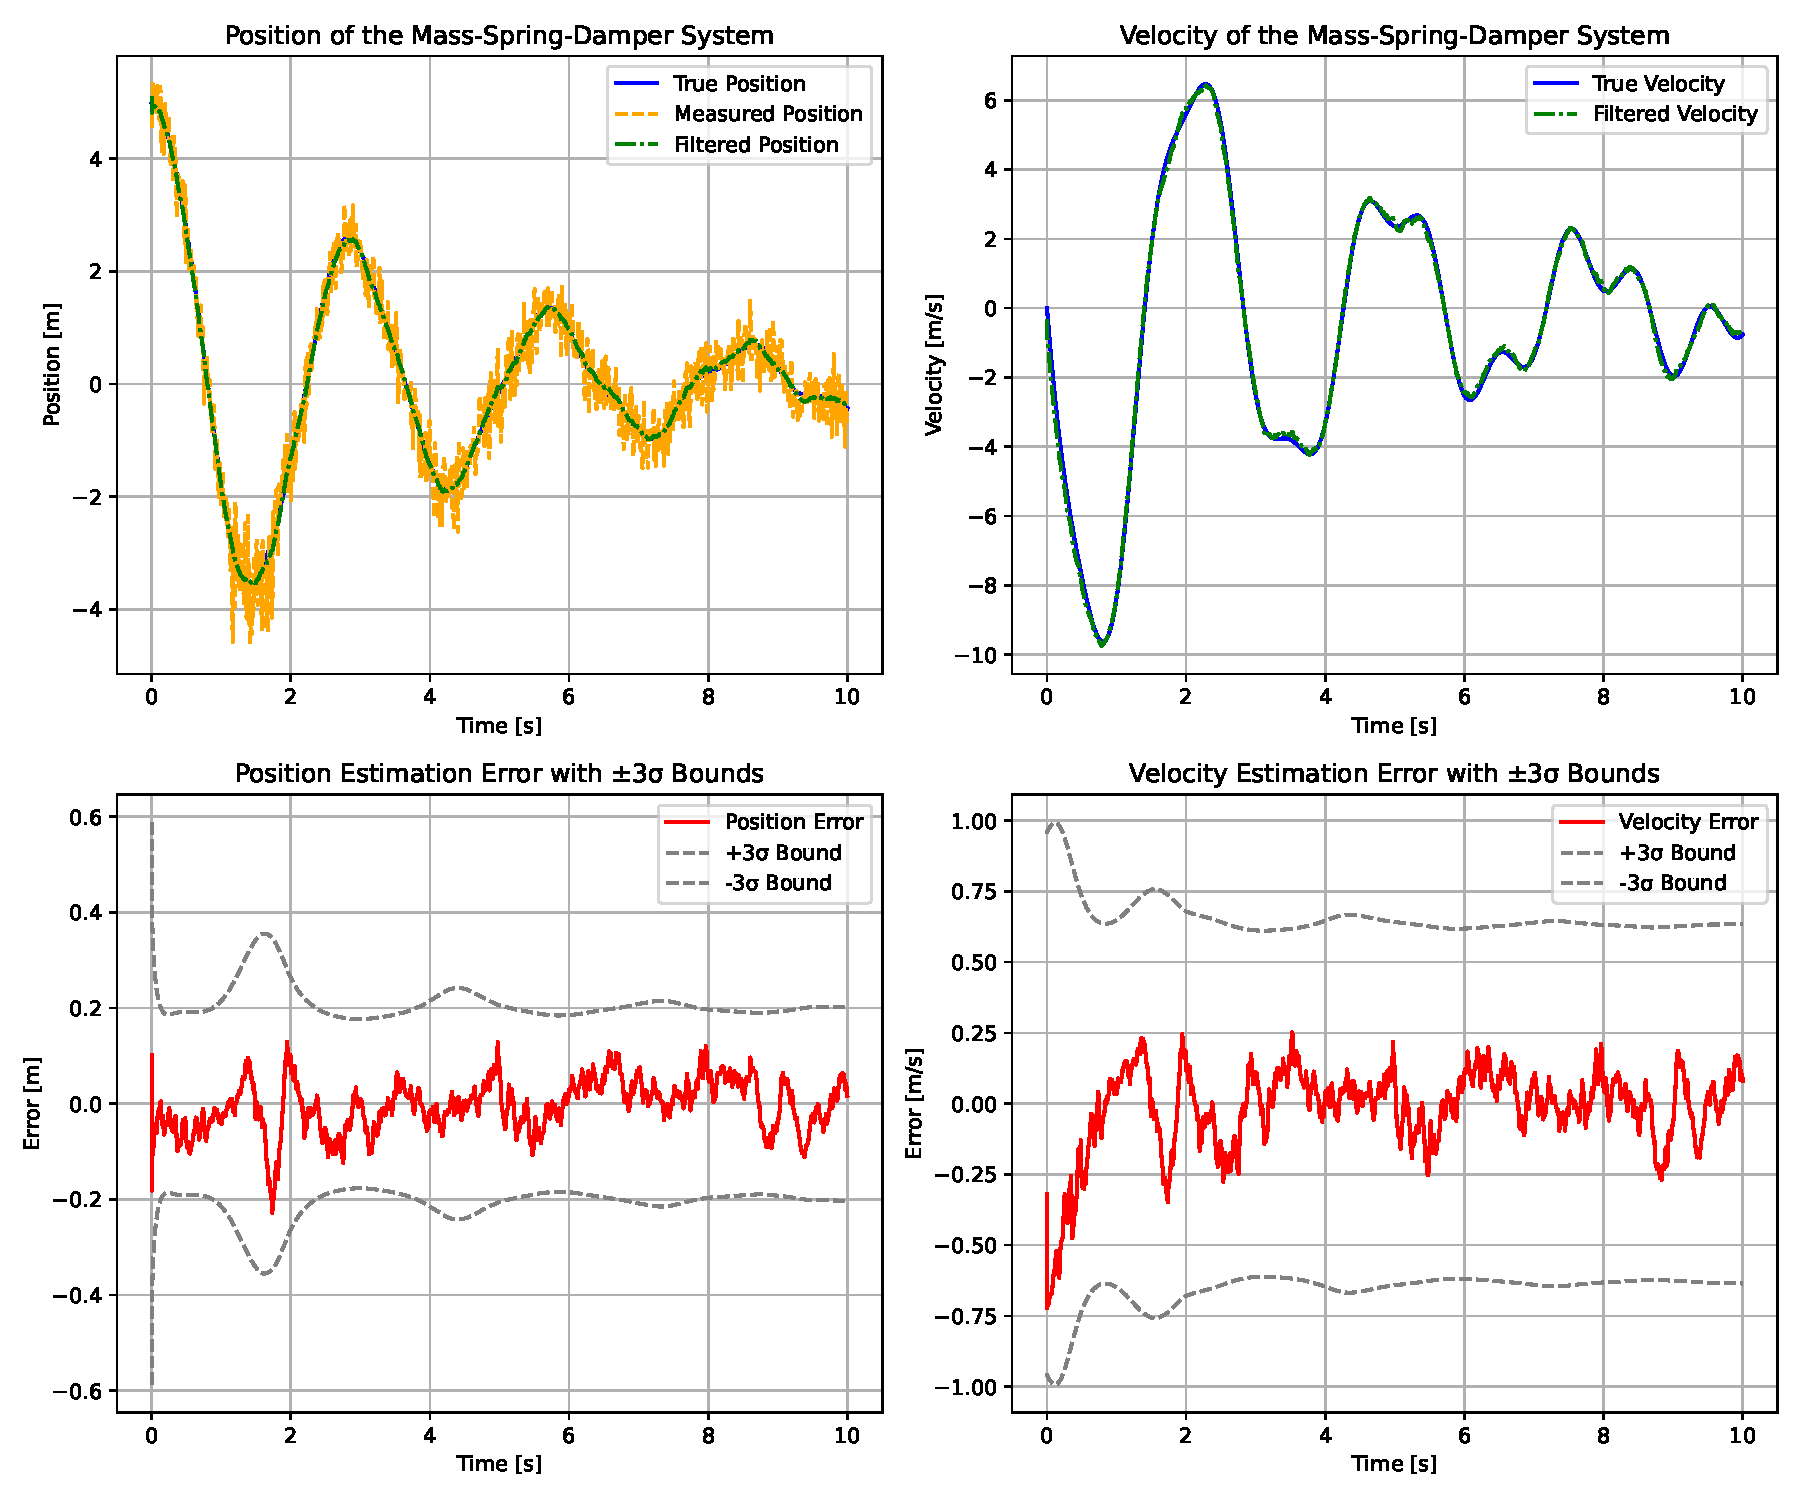
\includegraphics[width=1\textwidth]{figures/ekf.pdf}
    \caption{Extended Kalman filter estimation where the measurement is the Euclidean distance to a fixed point on the wall. The plots show the true, estimated, and measured values along with the estimation errors and \( \pm 3\sigma \) bounds.}
    \label{fig:ekf}
\end{figure}





\printbibliography        % Prints the references with BibLaTeX

\end{document}